% Options for packages loaded elsewhere
\PassOptionsToPackage{unicode}{hyperref}
\PassOptionsToPackage{hyphens}{url}
%
\documentclass[
]{book}
\usepackage{lmodern}
\usepackage{amssymb,amsmath}
\usepackage{ifxetex,ifluatex}
\ifnum 0\ifxetex 1\fi\ifluatex 1\fi=0 % if pdftex
  \usepackage[T1]{fontenc}
  \usepackage[utf8]{inputenc}
  \usepackage{textcomp} % provide euro and other symbols
\else % if luatex or xetex
  \usepackage{unicode-math}
  \defaultfontfeatures{Scale=MatchLowercase}
  \defaultfontfeatures[\rmfamily]{Ligatures=TeX,Scale=1}
\fi
% Use upquote if available, for straight quotes in verbatim environments
\IfFileExists{upquote.sty}{\usepackage{upquote}}{}
\IfFileExists{microtype.sty}{% use microtype if available
  \usepackage[]{microtype}
  \UseMicrotypeSet[protrusion]{basicmath} % disable protrusion for tt fonts
}{}
\makeatletter
\@ifundefined{KOMAClassName}{% if non-KOMA class
  \IfFileExists{parskip.sty}{%
    \usepackage{parskip}
  }{% else
    \setlength{\parindent}{0pt}
    \setlength{\parskip}{6pt plus 2pt minus 1pt}}
}{% if KOMA class
  \KOMAoptions{parskip=half}}
\makeatother
\usepackage{xcolor}
\IfFileExists{xurl.sty}{\usepackage{xurl}}{} % add URL line breaks if available
\IfFileExists{bookmark.sty}{\usepackage{bookmark}}{\usepackage{hyperref}}
\hypersetup{
  pdftitle={Formato del TFG},
  pdfauthor={Marco Pérez Castro},
  hidelinks,
  pdfcreator={LaTeX via pandoc}}
\urlstyle{same} % disable monospaced font for URLs
\usepackage{color}
\usepackage{fancyvrb}
\newcommand{\VerbBar}{|}
\newcommand{\VERB}{\Verb[commandchars=\\\{\}]}
\DefineVerbatimEnvironment{Highlighting}{Verbatim}{commandchars=\\\{\}}
% Add ',fontsize=\small' for more characters per line
\usepackage{framed}
\definecolor{shadecolor}{RGB}{248,248,248}
\newenvironment{Shaded}{\begin{snugshade}}{\end{snugshade}}
\newcommand{\AlertTok}[1]{\textcolor[rgb]{0.94,0.16,0.16}{#1}}
\newcommand{\AnnotationTok}[1]{\textcolor[rgb]{0.56,0.35,0.01}{\textbf{\textit{#1}}}}
\newcommand{\AttributeTok}[1]{\textcolor[rgb]{0.77,0.63,0.00}{#1}}
\newcommand{\BaseNTok}[1]{\textcolor[rgb]{0.00,0.00,0.81}{#1}}
\newcommand{\BuiltInTok}[1]{#1}
\newcommand{\CharTok}[1]{\textcolor[rgb]{0.31,0.60,0.02}{#1}}
\newcommand{\CommentTok}[1]{\textcolor[rgb]{0.56,0.35,0.01}{\textit{#1}}}
\newcommand{\CommentVarTok}[1]{\textcolor[rgb]{0.56,0.35,0.01}{\textbf{\textit{#1}}}}
\newcommand{\ConstantTok}[1]{\textcolor[rgb]{0.00,0.00,0.00}{#1}}
\newcommand{\ControlFlowTok}[1]{\textcolor[rgb]{0.13,0.29,0.53}{\textbf{#1}}}
\newcommand{\DataTypeTok}[1]{\textcolor[rgb]{0.13,0.29,0.53}{#1}}
\newcommand{\DecValTok}[1]{\textcolor[rgb]{0.00,0.00,0.81}{#1}}
\newcommand{\DocumentationTok}[1]{\textcolor[rgb]{0.56,0.35,0.01}{\textbf{\textit{#1}}}}
\newcommand{\ErrorTok}[1]{\textcolor[rgb]{0.64,0.00,0.00}{\textbf{#1}}}
\newcommand{\ExtensionTok}[1]{#1}
\newcommand{\FloatTok}[1]{\textcolor[rgb]{0.00,0.00,0.81}{#1}}
\newcommand{\FunctionTok}[1]{\textcolor[rgb]{0.00,0.00,0.00}{#1}}
\newcommand{\ImportTok}[1]{#1}
\newcommand{\InformationTok}[1]{\textcolor[rgb]{0.56,0.35,0.01}{\textbf{\textit{#1}}}}
\newcommand{\KeywordTok}[1]{\textcolor[rgb]{0.13,0.29,0.53}{\textbf{#1}}}
\newcommand{\NormalTok}[1]{#1}
\newcommand{\OperatorTok}[1]{\textcolor[rgb]{0.81,0.36,0.00}{\textbf{#1}}}
\newcommand{\OtherTok}[1]{\textcolor[rgb]{0.56,0.35,0.01}{#1}}
\newcommand{\PreprocessorTok}[1]{\textcolor[rgb]{0.56,0.35,0.01}{\textit{#1}}}
\newcommand{\RegionMarkerTok}[1]{#1}
\newcommand{\SpecialCharTok}[1]{\textcolor[rgb]{0.00,0.00,0.00}{#1}}
\newcommand{\SpecialStringTok}[1]{\textcolor[rgb]{0.31,0.60,0.02}{#1}}
\newcommand{\StringTok}[1]{\textcolor[rgb]{0.31,0.60,0.02}{#1}}
\newcommand{\VariableTok}[1]{\textcolor[rgb]{0.00,0.00,0.00}{#1}}
\newcommand{\VerbatimStringTok}[1]{\textcolor[rgb]{0.31,0.60,0.02}{#1}}
\newcommand{\WarningTok}[1]{\textcolor[rgb]{0.56,0.35,0.01}{\textbf{\textit{#1}}}}
\usepackage{longtable,booktabs}
% Correct order of tables after \paragraph or \subparagraph
\usepackage{etoolbox}
\makeatletter
\patchcmd\longtable{\par}{\if@noskipsec\mbox{}\fi\par}{}{}
\makeatother
% Allow footnotes in longtable head/foot
\IfFileExists{footnotehyper.sty}{\usepackage{footnotehyper}}{\usepackage{footnote}}
\makesavenoteenv{longtable}
\usepackage{graphicx}
\makeatletter
\def\maxwidth{\ifdim\Gin@nat@width>\linewidth\linewidth\else\Gin@nat@width\fi}
\def\maxheight{\ifdim\Gin@nat@height>\textheight\textheight\else\Gin@nat@height\fi}
\makeatother
% Scale images if necessary, so that they will not overflow the page
% margins by default, and it is still possible to overwrite the defaults
% using explicit options in \includegraphics[width, height, ...]{}
\setkeys{Gin}{width=\maxwidth,height=\maxheight,keepaspectratio}
% Set default figure placement to htbp
\makeatletter
\def\fps@figure{htbp}
\makeatother
\usepackage[normalem]{ulem}
% Avoid problems with \sout in headers with hyperref
\pdfstringdefDisableCommands{\renewcommand{\sout}{}}
\setlength{\emergencystretch}{3em} % prevent overfull lines
\providecommand{\tightlist}{%
  \setlength{\itemsep}{0pt}\setlength{\parskip}{0pt}}
\setcounter{secnumdepth}{5}
\usepackage{booktabs}
\ifluatex
  \usepackage{selnolig}  % disable illegal ligatures
\fi
\usepackage[]{natbib}
\bibliographystyle{apalike}

\title{Formato del TFG}
\author{Marco Pérez Castro}
\date{2020-11-06}

\begin{document}
\maketitle

{
\setcounter{tocdepth}{1}
\tableofcontents
}
\hypertarget{requisitos-previos}{%
\chapter{Requisitos previos}\label{requisitos-previos}}

Esto es un documento de prueba escrito en \textbf{Markdown}. Podemos escribir cualquier cosa que soporte Pandoc's Markdown, por ejemplo, fórmulas matemáticas \(\int x dx = \frac{x^2}{2}+c\)

El paquete \textbf{bookdown} se puede instalar desde el CRAN o Github:

\begin{Shaded}
\begin{Highlighting}[]
\FunctionTok{install.packages}\NormalTok{(}\StringTok{"bookdown"}\NormalTok{)}
\end{Highlighting}
\end{Shaded}

\hypertarget{intro}{%
\chapter{Introducción}\label{intro}}

Podemos etiquetar capítulos y secciones usando \texttt{\{\#label\}} detrás de ellos. Por ejemplo, puedo hacer referencia al Capítulo \ref{intro}. Si no se etiquetan se le asignará una etiqueta automática de todas formas, por ejemplo \ref{python}.

Figuras y tablas con pie de imagen serán colocadas en entornos \texttt{figure} y \texttt{table} respectivamente.

\begin{Shaded}
\begin{Highlighting}[]
\FunctionTok{par}\NormalTok{(}\AttributeTok{mar =} \FunctionTok{c}\NormalTok{(}\DecValTok{4}\NormalTok{, }\DecValTok{4}\NormalTok{, .}\DecValTok{1}\NormalTok{, .}\DecValTok{1}\NormalTok{))}
\FunctionTok{plot}\NormalTok{(pressure, }\AttributeTok{type =} \StringTok{\textquotesingle{}b\textquotesingle{}}\NormalTok{, }\AttributeTok{pch =} \DecValTok{19}\NormalTok{)}
\end{Highlighting}
\end{Shaded}

\begin{figure}

{\centering 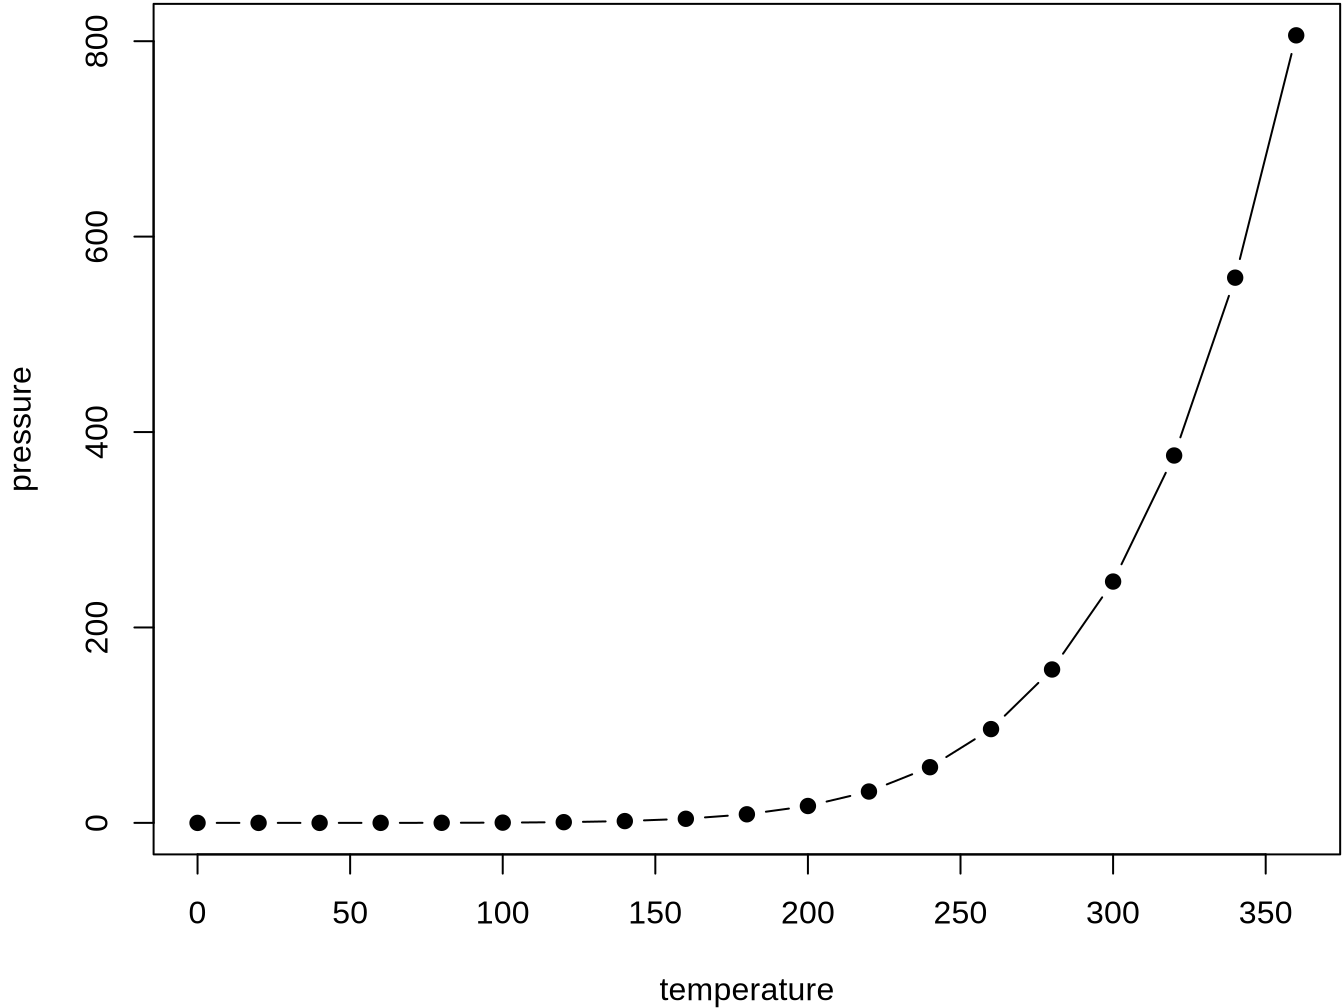
\includegraphics[width=0.8\linewidth]{Test_files/figure-latex/graf-imp-1} 

}

\caption{Gráfica muy importante}\label{fig:graf-imp}
\end{figure}

Se puede hacer referencia a una figura por su etiqueta del bloque de código usando el prefijo \texttt{fig:},por ejemplo, ver figura \ref{fig:graf-imp}. Análogamente, podemos referenciar tablas generadas por \texttt{knitr::kable()}, por ejemplo, ver tabla @ref(tab:tab-imp

\begin{Shaded}
\begin{Highlighting}[]
\NormalTok{knitr}\SpecialCharTok{::}\FunctionTok{kable}\NormalTok{(}
  \FunctionTok{head}\NormalTok{(iris, }\DecValTok{20}\NormalTok{), }\AttributeTok{caption =} \StringTok{\textquotesingle{}Tabla muy importante\textquotesingle{}}\NormalTok{,}
  \AttributeTok{booktabs =} \ConstantTok{TRUE}
\NormalTok{)}
\end{Highlighting}
\end{Shaded}

\begin{table}

\caption{\label{tab:tab-imp}Tabla muy importante}
\centering
\begin{tabular}[t]{rrrrl}
\toprule
Sepal.Length & Sepal.Width & Petal.Length & Petal.Width & Species\\
\midrule
5.1 & 3.5 & 1.4 & 0.2 & setosa\\
4.9 & 3.0 & 1.4 & 0.2 & setosa\\
4.7 & 3.2 & 1.3 & 0.2 & setosa\\
4.6 & 3.1 & 1.5 & 0.2 & setosa\\
5.0 & 3.6 & 1.4 & 0.2 & setosa\\
\addlinespace
5.4 & 3.9 & 1.7 & 0.4 & setosa\\
4.6 & 3.4 & 1.4 & 0.3 & setosa\\
5.0 & 3.4 & 1.5 & 0.2 & setosa\\
4.4 & 2.9 & 1.4 & 0.2 & setosa\\
4.9 & 3.1 & 1.5 & 0.1 & setosa\\
\addlinespace
5.4 & 3.7 & 1.5 & 0.2 & setosa\\
4.8 & 3.4 & 1.6 & 0.2 & setosa\\
4.8 & 3.0 & 1.4 & 0.1 & setosa\\
4.3 & 3.0 & 1.1 & 0.1 & setosa\\
5.8 & 4.0 & 1.2 & 0.2 & setosa\\
\addlinespace
5.7 & 4.4 & 1.5 & 0.4 & setosa\\
5.4 & 3.9 & 1.3 & 0.4 & setosa\\
5.1 & 3.5 & 1.4 & 0.3 & setosa\\
5.7 & 3.8 & 1.7 & 0.3 & setosa\\
5.1 & 3.8 & 1.5 & 0.3 & setosa\\
\bottomrule
\end{tabular}
\end{table}

Tambien podemos añadir menciones. Por ejemplo, estamos usando el paquete \textbf{bookdown} \citep{R-bookdown} en este libro de prueba, el cual ha sido construido sobre R Markdown y \textbf{knitr} \citep{xie2015}.

\hypertarget{test}{%
\chapter{Test}\label{test}}

Aquí tenemos un capítulo muy importante.

\hypertarget{otro-test}{%
\chapter{Otro test}\label{otro-test}}

Este capítulo es todavía mas importante que el anterior.

\hypertarget{modelos-y-aplicaciones}{%
\chapter{Modelos y aplicaciones}\label{modelos-y-aplicaciones}}

Probaremos algunas aplicaciones \emph{significativas} a lo largo de este capítulo.

\hypertarget{ejemplo-uno}{%
\section{Ejemplo uno}\label{ejemplo-uno}}

\hypertarget{ejemplo-dos}{%
\section{Ejemplo dos}\label{ejemplo-dos}}

\hypertarget{python}{%
\chapter{Python}\label{python}}

Como seguimos trabajando con \emph{RStudio}, cargando la librería \texttt{reticulate} obtenemos toda la artillería de Python a nuestra disposición:

\begin{Shaded}
\begin{Highlighting}[]
\FunctionTok{library}\NormalTok{(reticulate)}
\end{Highlighting}
\end{Shaded}

\begin{Shaded}
\begin{Highlighting}[]
\ImportTok{from}\NormalTok{ mpl\_toolkits.mplot3d }\ImportTok{import}\NormalTok{ Axes3D}
\ImportTok{import}\NormalTok{ numpy }\ImportTok{as}\NormalTok{ np}
\ImportTok{import}\NormalTok{ matplotlib.pyplot }\ImportTok{as}\NormalTok{ plt}
\ImportTok{from}\NormalTok{ matplotlib }\ImportTok{import}\NormalTok{ cm}
\ImportTok{from}\NormalTok{ matplotlib.ticker }\ImportTok{import}\NormalTok{ LinearLocator, FormatStrFormatter}
\NormalTok{fig }\OperatorTok{=}\NormalTok{ plt.figure()}
\NormalTok{ax }\OperatorTok{=}\NormalTok{ fig.gca(projection}\OperatorTok{=}\StringTok{\textquotesingle{}3d\textquotesingle{}}\NormalTok{)}
\NormalTok{X }\OperatorTok{=}\NormalTok{ np.arange(}\OperatorTok{{-}}\DecValTok{5}\NormalTok{, }\DecValTok{5}\NormalTok{, }\FloatTok{0.25}\NormalTok{)}
\NormalTok{Y }\OperatorTok{=}\NormalTok{ np.arange(}\OperatorTok{{-}}\DecValTok{5}\NormalTok{, }\DecValTok{5}\NormalTok{, }\FloatTok{0.25}\NormalTok{)}
\NormalTok{X, Y }\OperatorTok{=}\NormalTok{ np.meshgrid(X, Y)}
\NormalTok{Z }\OperatorTok{=}\NormalTok{ np.sin(np.sqrt(X}\OperatorTok{**}\DecValTok{2} \OperatorTok{+}\NormalTok{ Y}\OperatorTok{**}\DecValTok{2}\NormalTok{))}
\NormalTok{surf }\OperatorTok{=}\NormalTok{ ax.plot\_surface(X, Y, Z, cmap}\OperatorTok{=}\NormalTok{cm.coolwarm,}
\NormalTok{        linewidth}\OperatorTok{=}\DecValTok{0}\NormalTok{, antialiased}\OperatorTok{=}\VariableTok{False}\NormalTok{)}
\NormalTok{fig.colorbar(surf, shrink}\OperatorTok{=}\FloatTok{0.5}\NormalTok{, aspect}\OperatorTok{=}\DecValTok{5}\NormalTok{)}\OperatorTok{;}
\NormalTok{plt.show()                                }
\end{Highlighting}
\end{Shaded}

\begin{figure}

{\centering 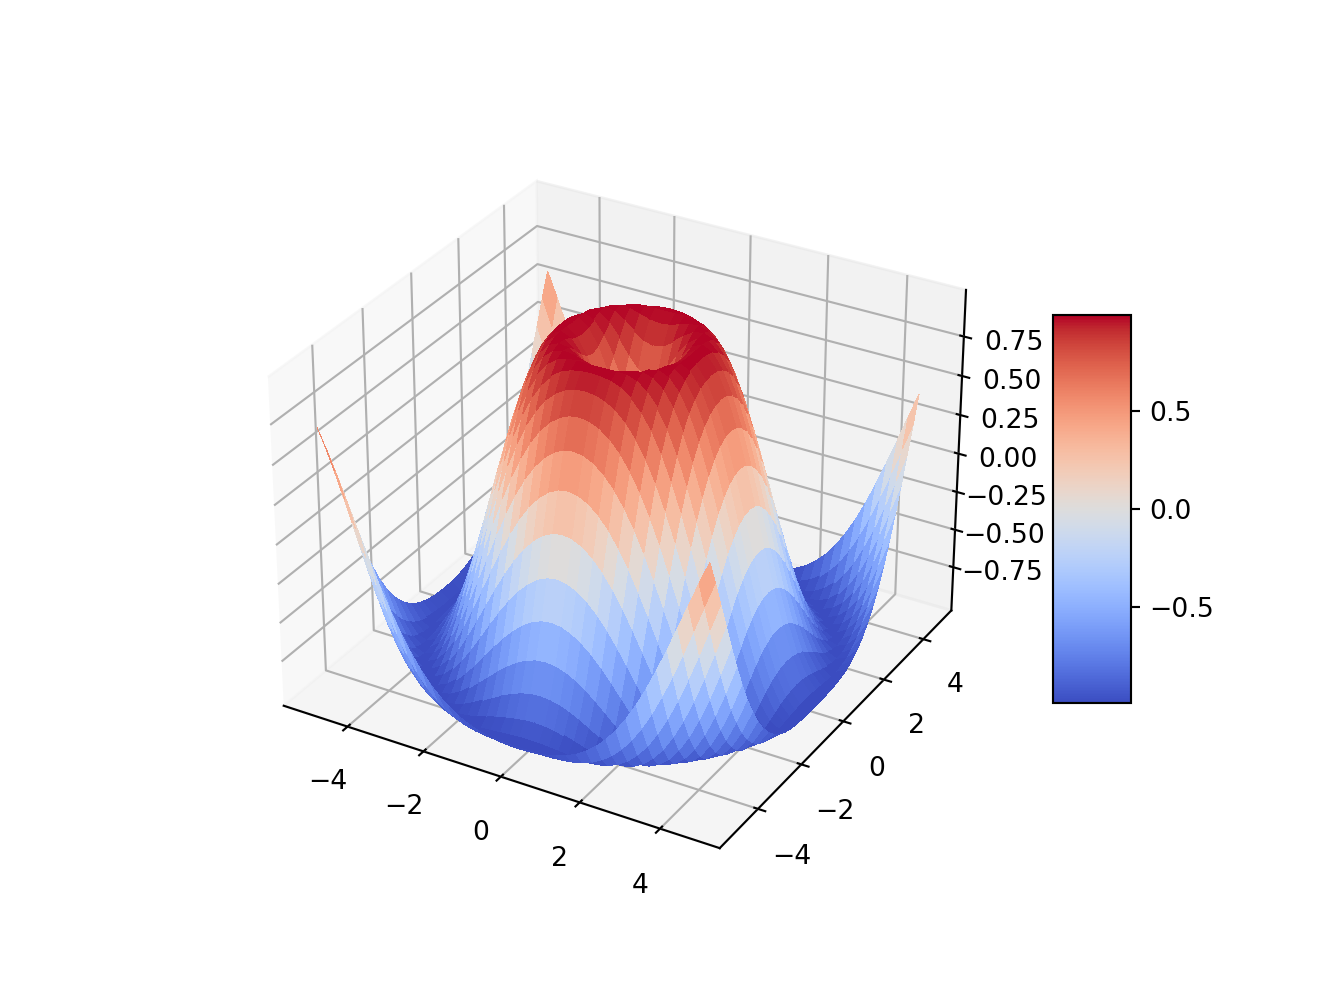
\includegraphics[width=0.8\linewidth]{Test_files/figure-latex/unnamed-chunk-3-1} 

}

\caption{Gráfica clave de Python}\label{fig:unnamed-chunk-3}
\end{figure}

\hypertarget{hoja-de-ruta}{%
\chapter{Hoja de ruta}\label{hoja-de-ruta}}

\begin{itemize}
\tightlist
\item
  Añadir referencias correctamente.
\item
  \sout{Cambiar o quitar los iconos de las redes sociales en la esquina superior derecha.}
\item
  Cambiar el resaltado de código de Python. Así se ve demasiado plano y resulta difícil leerlo.
\item
  Experimentar con paquetes de Latex.
\item
  \sout{Al compilar esta página tengo el siguiente error:
  \mbox{\texttt{/usr/lib64/R/bin/exec/R:\ symbol\ lookup\ error:\ /usr/lib/rstudio/plugins/imageformats/libqgif.so:\ undefined\ symbol:\ \_ZdlPvm,\ version\ Qt\_5}}
  Ese error me impide modificar el nombre que aparece encima del menú de navegación que hay a la izquierda y me da un warning en las referencias, aunque estas parecen funcionar más o menos bien. Es un problema de mi ordenador debido a un lío que tiene que haber en las librerías \emph{Qt}. Probaré con el sobremesa y espero que no tenga más problemas.}
\item
  Experimentar con el PDF autogenerado. Se ve muy cutre.
\item
  Cuando se le da a editar, que lleve a la página adecuada de Github para poder crear un request.
\item
  Probar los distintos temas de la página (tema claro u oscuro).
\item
  Icono web. Localmente me aparece, pero no aperece al subirlo.
\end{itemize}

  \bibliography{book.bib,packages.bib}

\end{document}
